% !TEX program = lualatex
% Final Y3 Individual Project Presentation
% Atilade Gabriel Oke — University of Manchester (EEE)
% Module: EEEN30330 | Compile: lualatex presentation.tex

\documentclass[aspectratio=169,11pt]{beamer}

% ---------- Packages ----------
\usepackage{fontspec}
\usepackage{amsmath,amssymb}
\usepackage{graphicx}
\usepackage{booktabs}
\usepackage{multirow}
\usepackage{array}
\usepackage{xcolor}
\usepackage{tikz}
\usetikzlibrary{arrows.meta,positioning,calc,fit,shapes.geometric}

\graphicspath{{figures/}}

% ---------- Theme ----------
\usetheme{metropolis}
\usecolortheme{default}

% Manchester palette
\definecolor{manpurple}{RGB}{96,37,121}
\definecolor{manpurple2}{RGB}{156,99,169}
\definecolor{manyellow}{RGB}{230,178,31}
\definecolor{slate}{RGB}{60,60,60}
\definecolor{accent}{RGB}{200,80,80}

\setbeamercolor{frametitle}{bg=manpurple,fg=white}
\setbeamercolor{title separator}{fg=manyellow}
\setbeamercolor{progress bar}{fg=manpurple,bg=manpurple2!30}
\setbeamercolor{alerted text}{fg=accent}
\setbeamercolor{block title}{bg=manpurple!15,fg=manpurple}
\setbeamercolor{block body}{bg=manpurple!5}

% Metropolis tweaks
\setbeamertemplate{frame numbering}[fraction]
\metroset{block=fill}
\metroset{subsectionpage=progressbar}

% ---------- Macros ----------
\newcommand{\NDR}{\mathrm{NDR}}
\newcommand{\Jfi}{\mathcal{J}}
\newcommand{\green}[1]{{\color{manpurple}\textbf{#1}}}
\newcommand{\red}[1]{{\color{accent}\textbf{#1}}}

% ---------- Title ----------
\title{Protocol-Aware Deep Reinforcement Learning for\\ Energy-Efficient UAV Data Collection in LoRaWAN}
\subtitle{EEEN30330 Individual 3rd-Year Project}
\author{Atilade Gabriel Oke}
\institute{Department of Electrical \& Electronic Engineering\\ The University of Manchester}
\date{Supervisor Review, April 2026}

% ==========================================================
\begin{document}
% ==========================================================

\maketitle

% ---------- Outline ----------
\begin{frame}{Overview}
    \tableofcontents
\end{frame}

% ==========================================================
\section{Motivation \& Objectives}
% ==========================================================

\begin{frame}{The Problem: SF Monoculture in Mobile UAV--LoRaWAN}
    \begin{columns}[T]
        \begin{column}{0.55\textwidth}
            \textbf{Scenario.} A UAV collects data from $N$ LoRa IoT sensors over a 2D
            area. Sensors share ISM bandwidth via orthogonal \textbf{Spreading Factors}
            (SF7--SF12).

            \medskip
            \textbf{Failure mode.} As the UAV moves, rapid RSSI changes force sensors
            to converge on the \emph{same} SF under LoRaWAN's Adaptive Data Rate
            (EMA-ADR, $\lambda{=}0.1$). Intra-SF collisions collapse throughput:
            the \alert{SF Monoculture}.

            \medskip
            \textbf{Gap.} Path planners ignore protocol physics; static protocol
            optimisers ignore UAV mobility. Neither solves the coupled problem.
        \end{column}
        \begin{column}{0.45\textwidth}
            \centering
            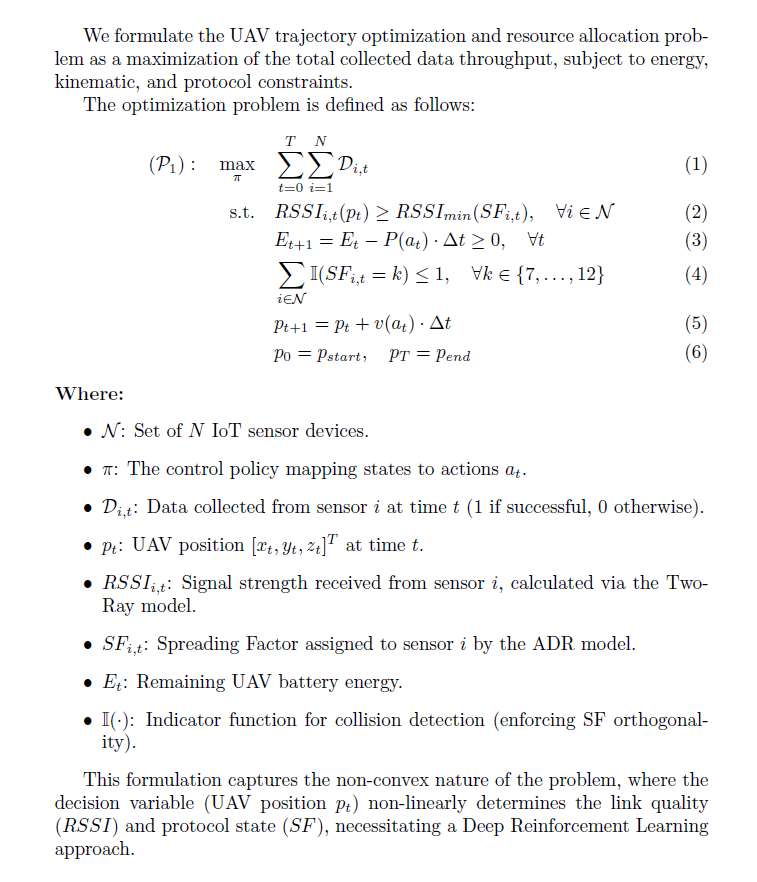
\includegraphics[width=\linewidth]{problem_formulation.png}
            {\scriptsize UAV over a LoRaWAN sensor field; link quality is a function of
            UAV position.}
        \end{column}
    \end{columns}
\end{frame}

\begin{frame}{Objectives}
    \begin{enumerate}
        \item \textbf{High-fidelity simulator.} First open Gymnasium environment to model
              the complete causal chain\\
              \quad UAV position $\to$ RSSI $\to$ EMA-ADR $\to$ Capture Effect
              $\to$ packet delivery.
        \item \textbf{POMDP formulation.} Multi-objective reward balancing energy,
              data freshness (AoI), and collection volume; Markov restoration via
              frame stacking.
        \item \textbf{DRL policy.} Train a Deep Q-Network that learns emergent
              protocol-aware flight, without hand-coded routing heuristics.
        \item \textbf{Baselines.} Evaluate against Nearest-Sensor Greedy,
              a novel \alert{SF-Aware Greedy}, and a \alert{TSP Oracle} upper bound.
        \item \textbf{Operational envelope.} Characterise feasibility across grid
              scales $100{\times}100 \to 1000{\times}1000$ and densities
              $N{\in}\{10,20,30,40\}$.
        \item \textbf{Statistical rigour.} Multi-seed ($n{=}20$) comparisons with
              Welch's $t$-test and Cohen's $d$.
    \end{enumerate}
\end{frame}

% ==========================================================
\section{Environment \& Problem Formulation}
% ==========================================================

\begin{frame}{Simulation Environment}
    \begin{columns}[T]
        \begin{column}{0.55\textwidth}
            \textbf{Physics.} Two-Ray Ground Reflection path-loss model, log-normal
            shadowing $\mathcal{N}(0, 4\,\text{dB})$, asynchronous duty cycles (eff.\ 10\% Tx
            probability), Capture Effect on same-SF collisions.

            \smallskip
            \textbf{Protocol.} EMA-ADR with smoothing $\lambda{=}0.1$
            $\Rightarrow$ SF update lag $\tau{=}10$ steps.

            \smallskip
            \textbf{Agent.} 100\,m altitude rotary-wing UAV, fixed battery,
            discrete cardinal actions $\{N,S,E,W,\text{Hover}\}$.

            \smallskip
            \textbf{Link budget.} SF12 ceiling
            $r_{\max}\approx 365$ grid units ($\approx 3{,}650$\,m) --- beyond this,
            UAV positioning genuinely matters.
        \end{column}
        \begin{column}{0.45\textwidth}
            \centering
            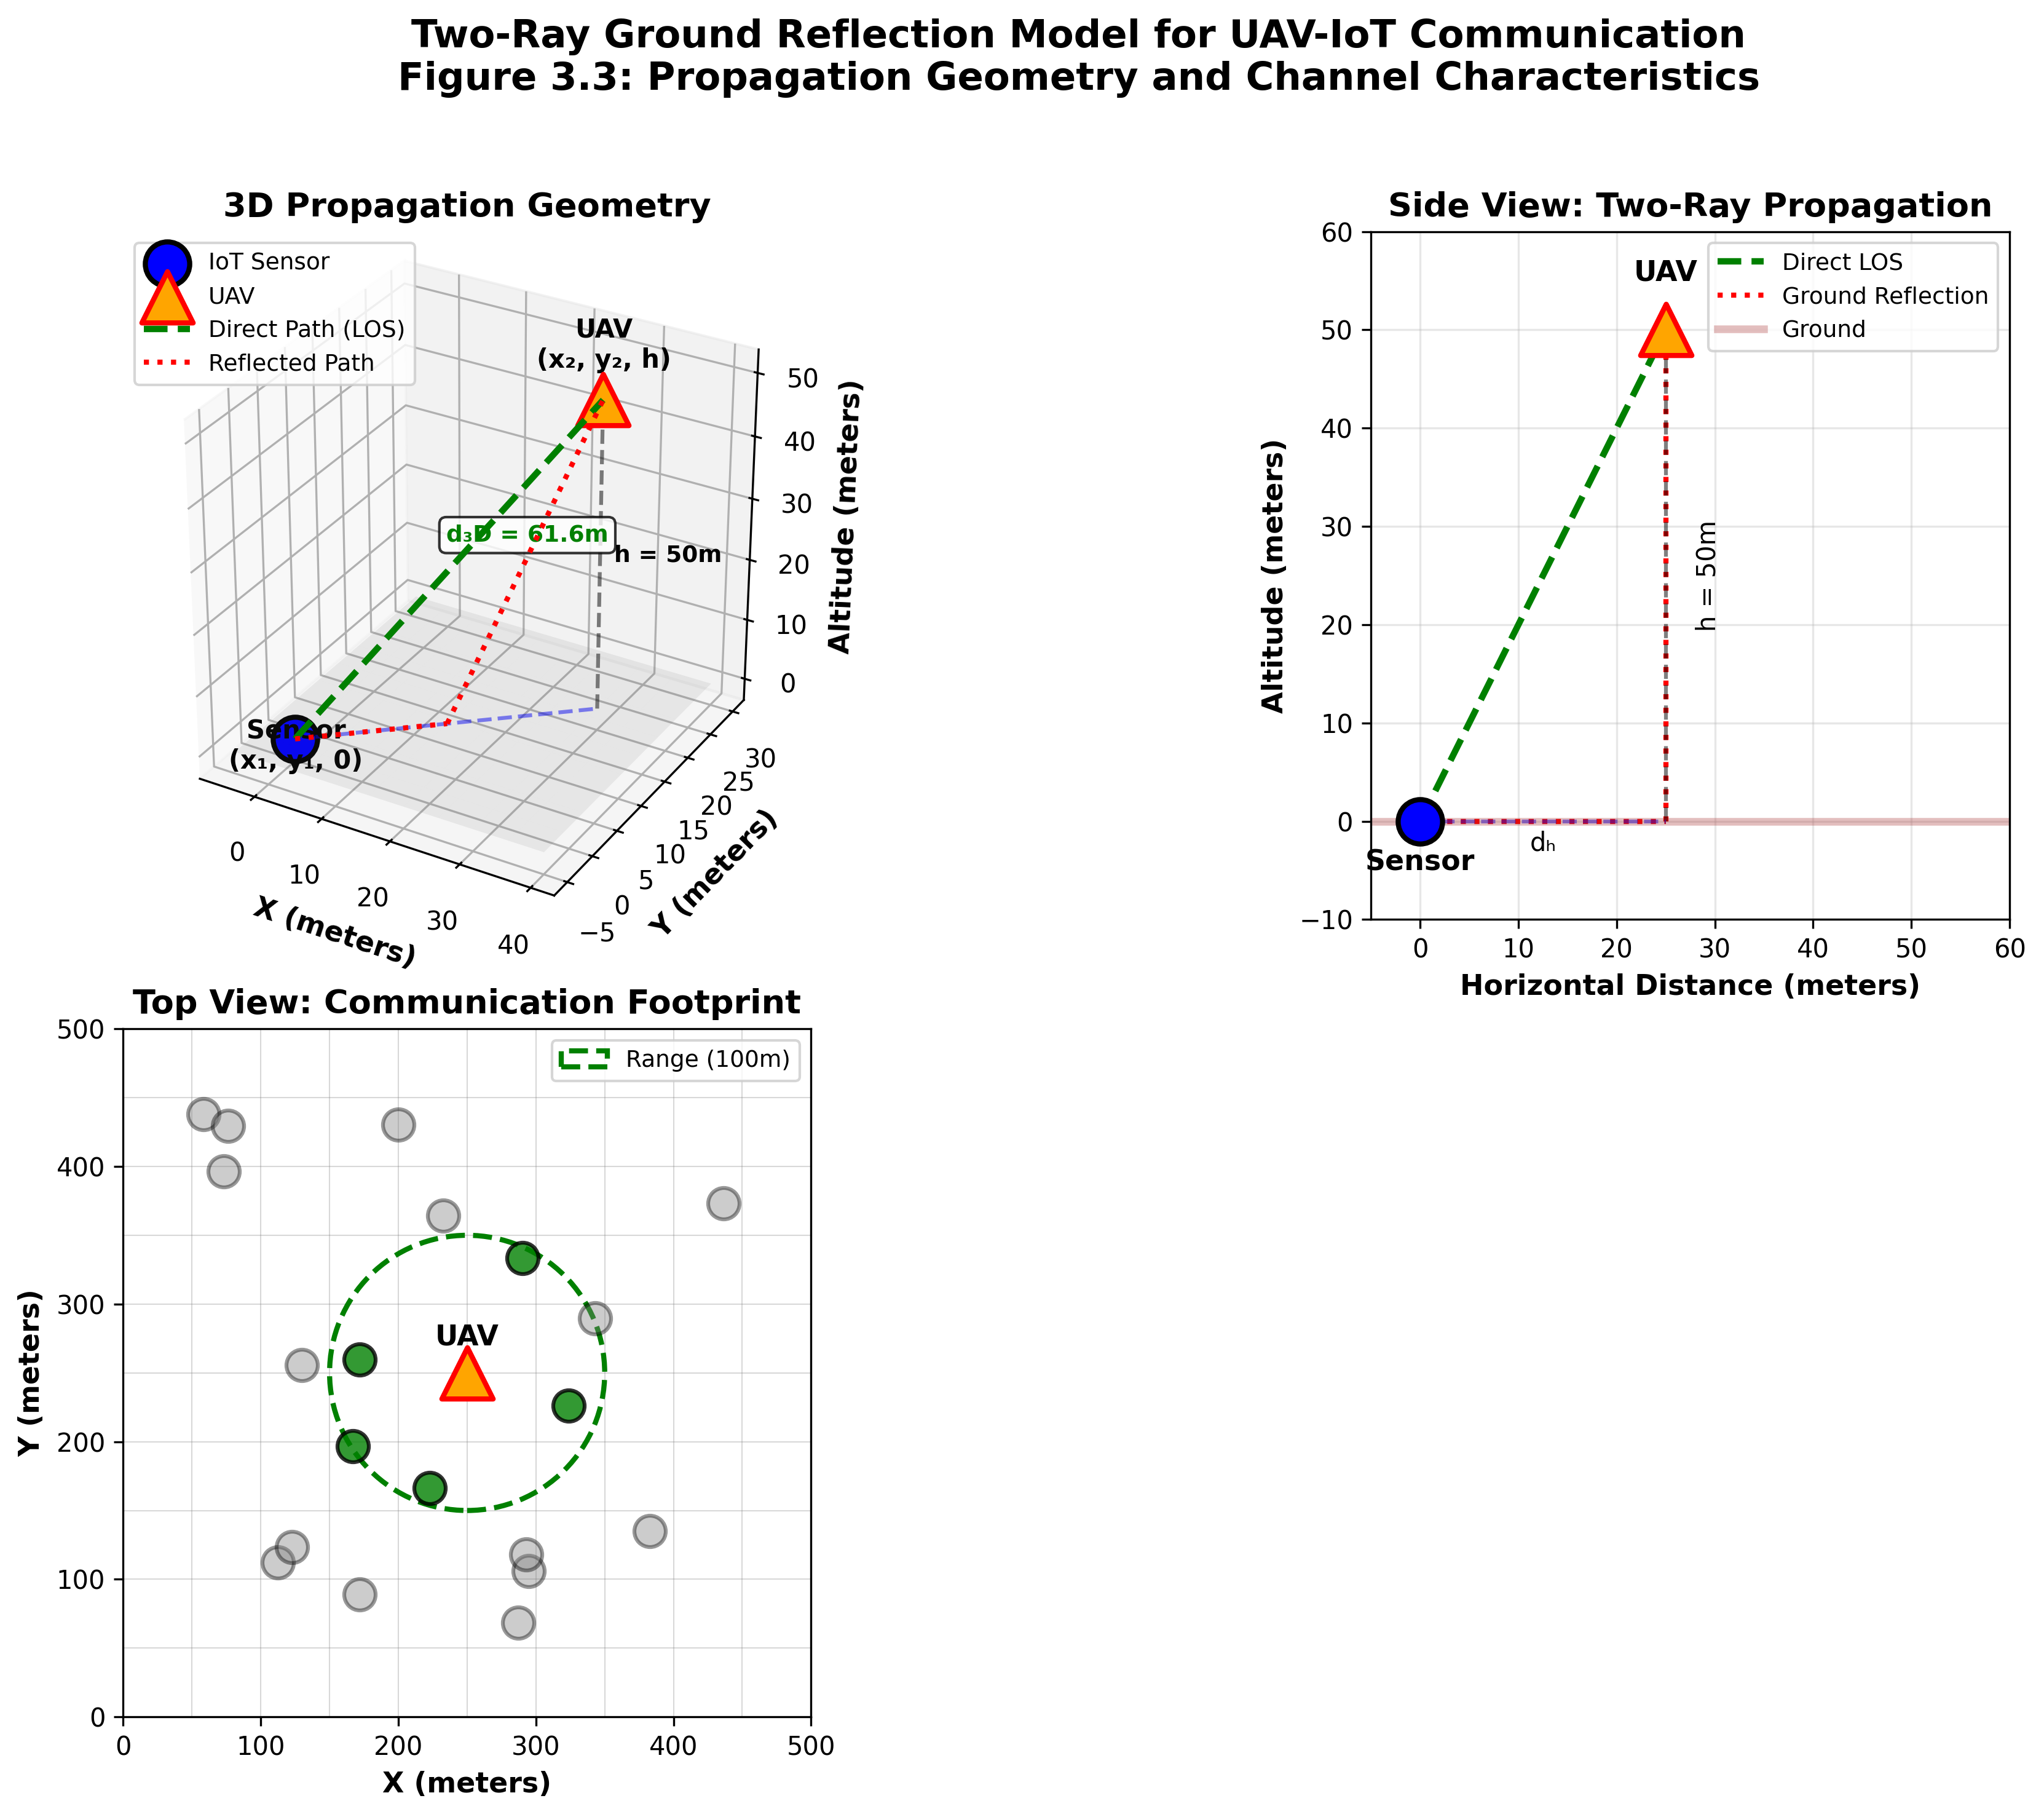
\includegraphics[width=\linewidth]{two_ray_model_3d.png}

            {\scriptsize Two-Ray propagation geometry: LoS + ground-reflected ray
            generate the grid-scale path-loss field.}
        \end{column}
    \end{columns}
\end{frame}

\begin{frame}{POMDP Formulation}
    \begin{block}{Objective (P1)}
        \vspace{-0.6em}
        \[
            \max_{\pi}\ \sum_{t=0}^{T}\sum_{i=1}^{N} D_{i,t}
            \quad\text{s.t.}\quad
            \underbrace{\text{RSSI}_{i,t}(p_t)\!\geq\! \text{RSSI}_{\min}(\text{SF}_{i,t})}_{\text{link budget}},\
            \underbrace{E_{t+1}\!\geq\!0}_{\text{energy}},\
            \underbrace{|\{i:\text{SF}_{i,t}{=}k\}|\!\leq\!1}_{\text{SF orthogonality}}
        \]
    \end{block}
    \textbf{Non-Markov coupling.} $p_t$ and $\text{SF}_{i,t}$ are coupled via EMA-ADR
    $\Rightarrow$ classical MILP/MPC cannot tractably encode history.

    \smallskip
    \textbf{State} (partial obs.): $\mathbf{S}_t = [p_t, E_t, B_t, U_t, Q_t] \in \mathbb{R}^{3+3N}$.\\
    \textbf{Markov restoration}: frame stacking $k{=}4$, so
    $\mathbf{S}_t^{\text{stk}} \in \mathbb{R}^{4(3+3N)}$ exposes EMA-ADR convergence.

    \smallskip
    \textbf{Reward.} Per-byte$\times$urgency, new-sensor bonus, urgency-reduction,
    starvation-variance penalty, terminal-unvisited penalty.
\end{frame}

% ==========================================================
\section{Agent \& Training}
% ==========================================================

\begin{frame}{DQN Architecture}
    \centering
    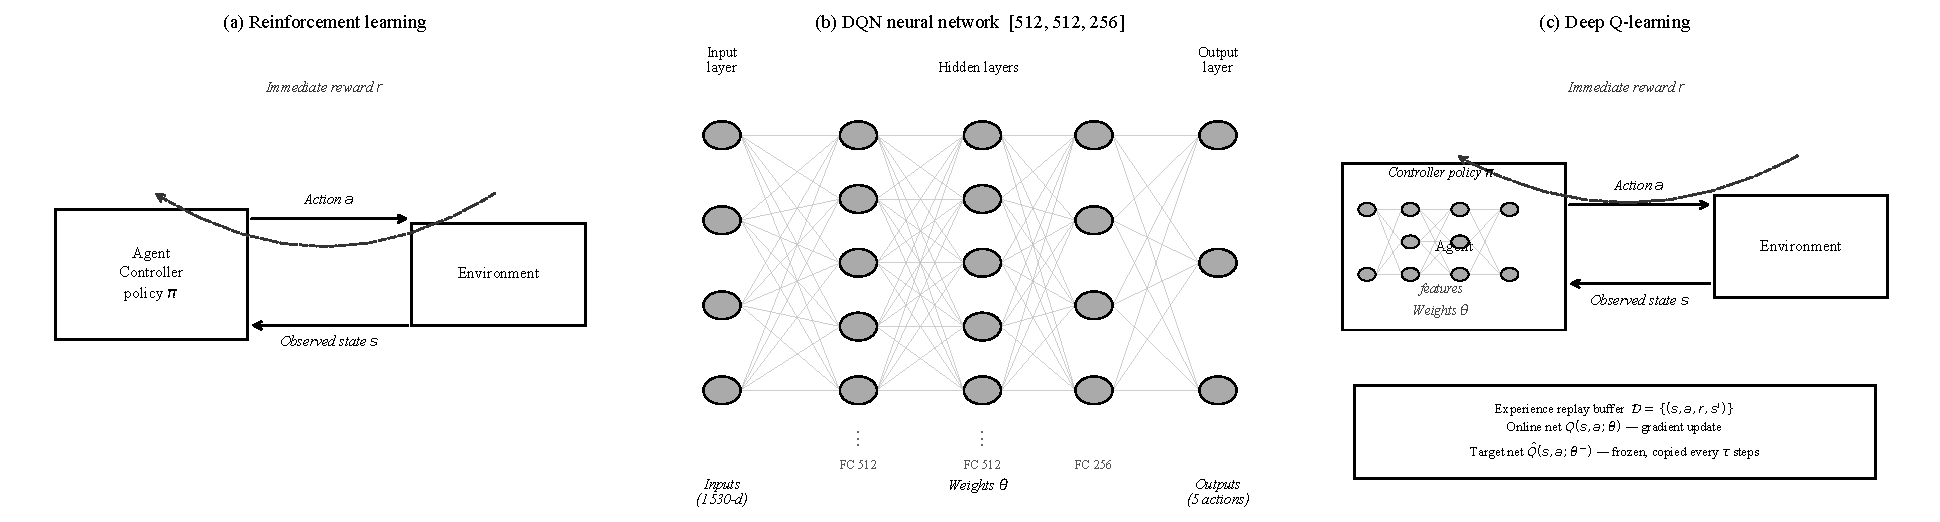
\includegraphics[width=0.92\textwidth]{drl_architecture.pdf}

    \smallskip
    \footnotesize
    \textbf{Backbone:} SB3 DQN, MLP $[512,512,256]$, ReLU, Adam
    ($lr{=}3{\times}10^{-4}$), $\gamma{=}0.99$. \quad
    \textbf{Replay:} 150k-transition buffer, batch $128$, target update every
    $1000$ steps. \quad
    \textbf{Exploration:} $\varepsilon{:}\,1.0{\to}0.05$ over $5\%$ of training. \quad
    \textbf{Horizon:} $T{=}2100$ steps ($\approx\!7$\,min).
\end{frame}

\begin{frame}{Training Regime --- Domain Randomisation + Curriculum}
    \begin{columns}[T]
        \begin{column}{0.55\textwidth}
            \textbf{Domain randomisation.} $4$ grid sizes $\times$ $4$ sensor counts
            $=$ \alert{16 conditions}, sampled uniformly per episode.

            \smallskip
            \textbf{Competence curriculum.} Advance to a denser stage only when
            a $50$-episode rolling window satisfies \emph{both}:
            \[
                \NDR \geq 95\%,\quad \Jfi \geq 0.85
            \]

            \smallskip
            \textbf{Parallelism.} $4$ env workers; PyTorch $2.7\,{+}\,$CUDA.

            \smallskip
            \textbf{Output.} A \alert{single} policy deployable over all
            $16$ conditions \emph{without} retraining.
        \end{column}
        \begin{column}{0.45\textwidth}
            \centering
            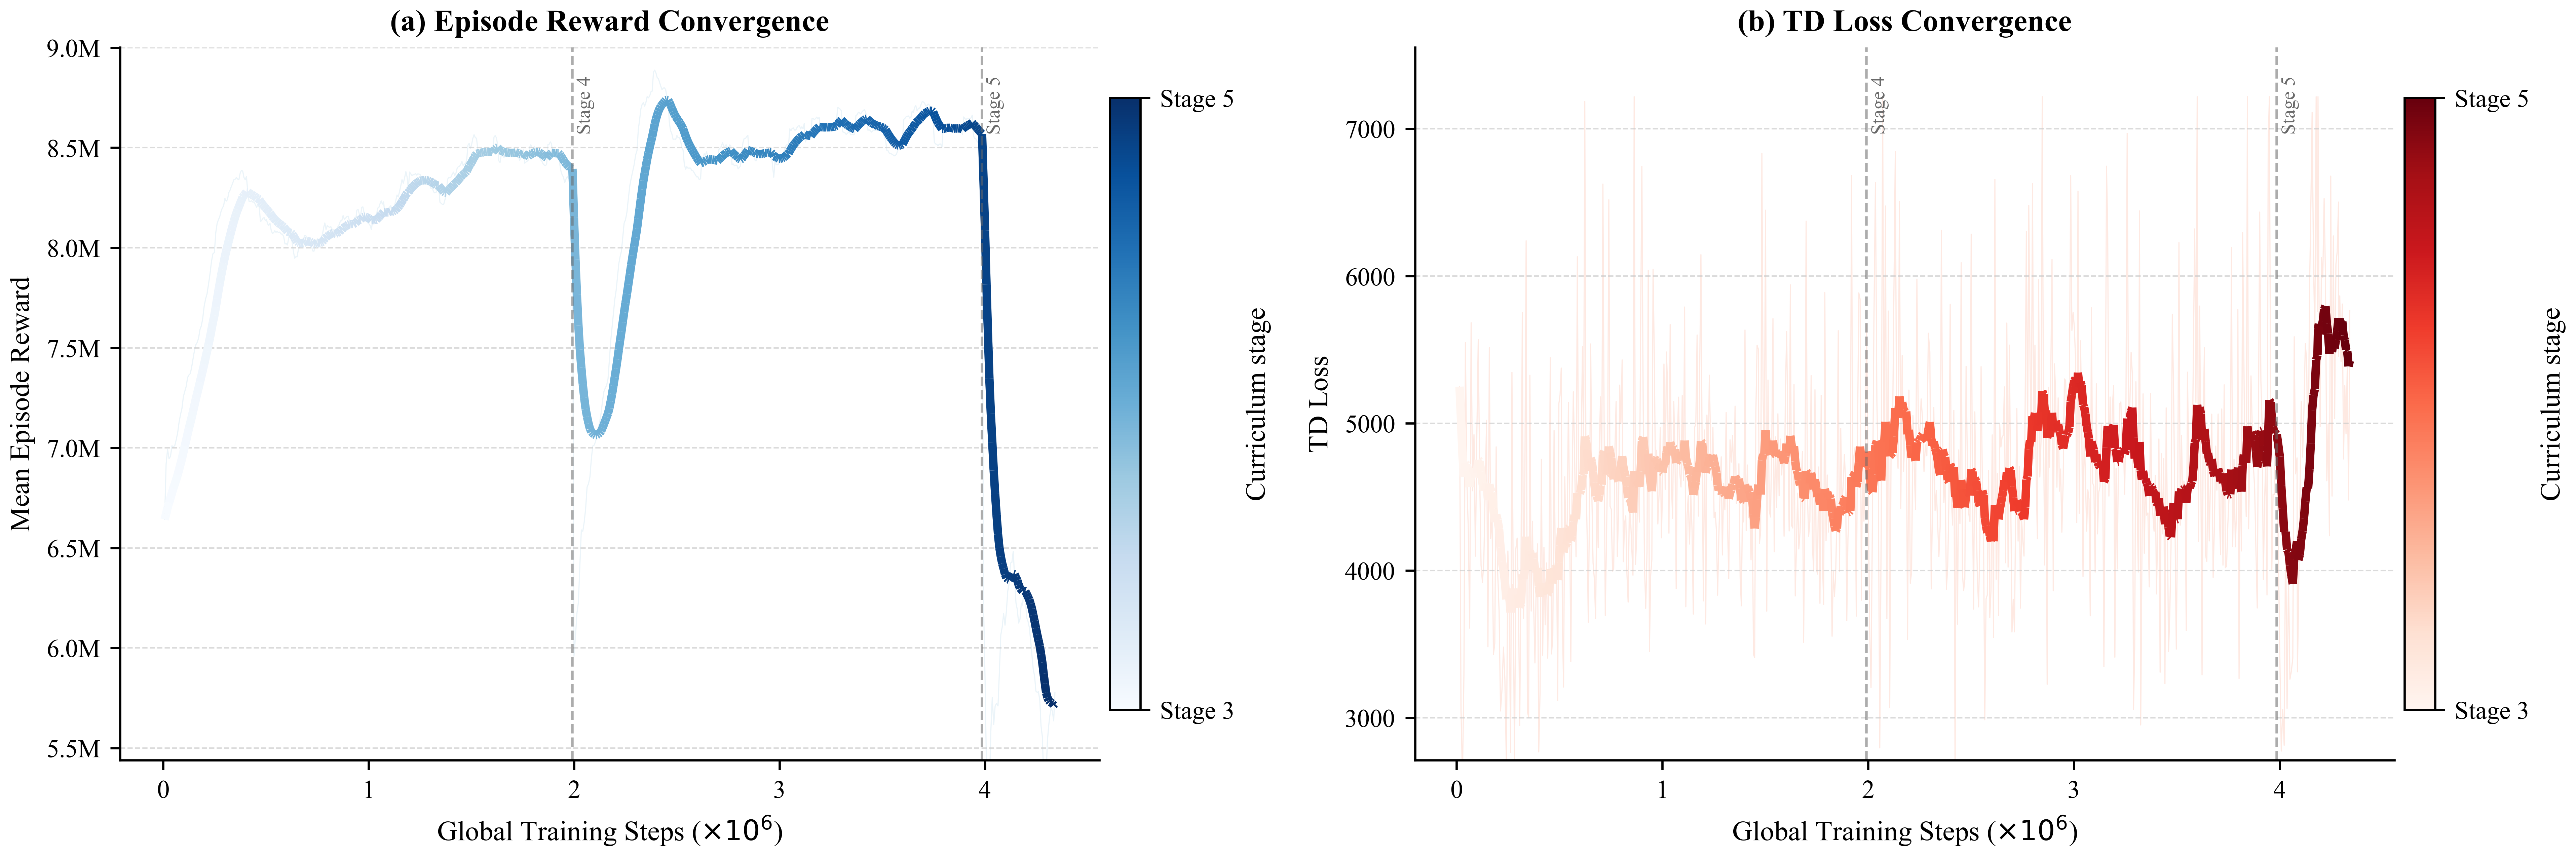
\includegraphics[width=\linewidth]{fig_training_convergence.png}\\
            {\scriptsize Competence-gated stage transitions; smooth convergence
            once the NDR/Jain gate fires.}
        \end{column}
    \end{columns}
\end{frame}

\begin{frame}{Baselines}
    \begin{description}[Nearest Greedy]
        \setlength{\itemsep}{0.6em}
        \item[\textbf{Nearest-Sensor Greedy}]
              At every step, move toward the closest sensor with a non-empty buffer.
              \emph{Protocol-blind.}
        \item[\textbf{SF-Aware Greedy} (novel)]
              Route toward the lowest-SF sensor with a non-empty buffer; ties broken
              by proximity. Encodes the very knowledge the DQN must \emph{learn}.
        \item[\textbf{TSP Oracle} (Nearest-Neighbour $+$ 2-opt)]
              Computes a distance-optimal tour over all sensors at episode start.
              \emph{Cheats by knowing sensor positions} $\Rightarrow$ distance ceiling, not
              a deployable controller.
    \end{description}

    \smallskip
    Evaluation: $n{=}20$ seeds per condition, reporting reward ($\times 10^6$), Jain's
    index $\Jfi$, efficiency (B/Wh), coverage; \alert{Welch's $t$-test} against the DQN.
\end{frame}

% ==========================================================
\section{Results}
% ==========================================================

\begin{frame}{Primary Result --- Statistical Parity with Greedy Baselines}
    \small
    \centering
    Primary condition: $N{=}20$ sensors, $500{\times}500$ grid, $n{=}20$ seeds.
    \begin{table}
    \begin{tabular}{lrrrr}
        \toprule
        Agent & Reward ($\times 10^6$) & $\Jfi$ & Eff.\ (B/Wh) & Coverage \\
        \midrule
        \textbf{DQN (ours)} & $5.58 \pm 0.57$ & $0.962 \pm 0.027$ & $188.5 \pm 18.4$ & \green{100\%}\\
        SF-Aware Greedy & $5.60 \pm 0.54$ & $0.963 \pm 0.026$ & $189.4 \pm 17.8$ & 100\%\\
        Nearest Greedy  & $5.60 \pm 0.58$ & $0.963 \pm 0.028$ & $189.2 \pm 18.9$ & 100\%\\
        \bottomrule
    \end{tabular}
    \end{table}
    \begin{itemize}\setlength\itemsep{0.3em}
        \item DQN vs.\ SF-Aware Greedy: $t = -0.157$, $p = \alert{0.876}$
        \item DQN vs.\ Nearest Greedy:\ \ $t = -0.140$, $p = \alert{0.889}$
    \end{itemize}
    \alert{No statistically significant difference} --- the learned policy reaches the
    heuristic ceiling \emph{without} hard-coded SF or proximity knowledge.
\end{frame}

\begin{frame}{Operational Envelope --- Scaling Reveals a Feasibility Ceiling}
    \small
    \begin{columns}[T]
        \begin{column}{0.52\textwidth}
            \begin{table}
            \centering
            \begin{tabular}{l l r r}
                \toprule
                Grid & Agent & $\Jfi$ & Eff.\ \\
                \midrule
                \multirow{3}{*}{$100^2$}
                 & DQN & 0.999 & 219.3\\
                 & SF-Aw. & 0.999 & 220.0\\
                 & Near. & 0.998 & 219.6\\
                \midrule
                \multirow{3}{*}{$300^2$}
                 & DQN & 0.999 & 221.5\\
                 & SF-Aw. & 0.999 & 220.9\\
                 & Near. & 0.999 & 221.3\\
                \midrule
                \multirow{3}{*}{$500^2$}
                 & DQN & 0.961 & 187.9\\
                 & SF-Aw. & 0.964 & 189.1\\
                 & Near. & 0.960 & 188.1\\
                \midrule
                \multirow{3}{*}{$1000^2$}
                 & DQN & 0.879 & 155.9\\
                 & SF-Aw. & 0.885 & 161.2\\
                 & Near. & 0.876 & 155.8\\
                \bottomrule
            \end{tabular}
            \end{table}
        \end{column}
        \begin{column}{0.48\textwidth}
            \textbf{Three regimes.}
            \begin{itemize}\setlength\itemsep{0.25em}
                \item \green{Trivial} ($\le 300^2$):\\ all agents $\Jfi\!\approx\!1.0$.
                \item \green{Feasible} ($500^2$):\\ resource contention onset;
                      DQN within 1.6\% of SFGreedy.
                \item \red{Infeasible} ($1000^2$):\\ diagonal $14{,}142$\,m
                      $>$ UAV budget\\ $\approx 15{,}782$\,m at 20\% reserve;\\
                      TSP tour $\approx 44{,}700$\,m $\Rightarrow$ \textbf{2.8${\times}$ over budget}.
            \end{itemize}
            \medskip
            \textbf{The binding constraint is physics, not policy.}
        \end{column}
    \end{columns}
\end{frame}

\begin{frame}{Emergent Behaviour --- Dwell-Then-Reposition}
    \begin{columns}[T]
        \begin{column}{0.58\textwidth}
            
\includegraphics[width=\linewidth]{agent_trajectories.png}
            {\scriptsize Four-agent trajectories on the same seed (SF-Aware,
            Nearest, DQN, TSP Oracle).}
        \end{column}
        \begin{column}{0.42\textwidth}
            \textbf{Qualitative signature.}
            \begin{itemize}\setlength\itemsep{0.2em}
                \item Greedy agents: near-straight sweeps sensor-to-sensor.
                \item \green{DQN:} deliberate \emph{repositioning} to points that place
                      multiple sensors within range across \emph{orthogonal} SFs.
                \item Devotes $2.9\%$ of steps to positioning moves
                      ($p{=}0.002$, $n{=}10$).
            \end{itemize}

            \medskip
            \textbf{Mechanism.} Dwell $\Rightarrow$ EMA-ADR drops SF
            $\Rightarrow$ higher Tx.

            \alert{Greedy look-ahead can't plan this.}
        \end{column}
    \end{columns}
\end{frame}

\begin{frame}{Emergent Behaviour --- SF Diversity Management}
    \begin{columns}[T]
        \begin{column}{0.5\textwidth}
            \centering
            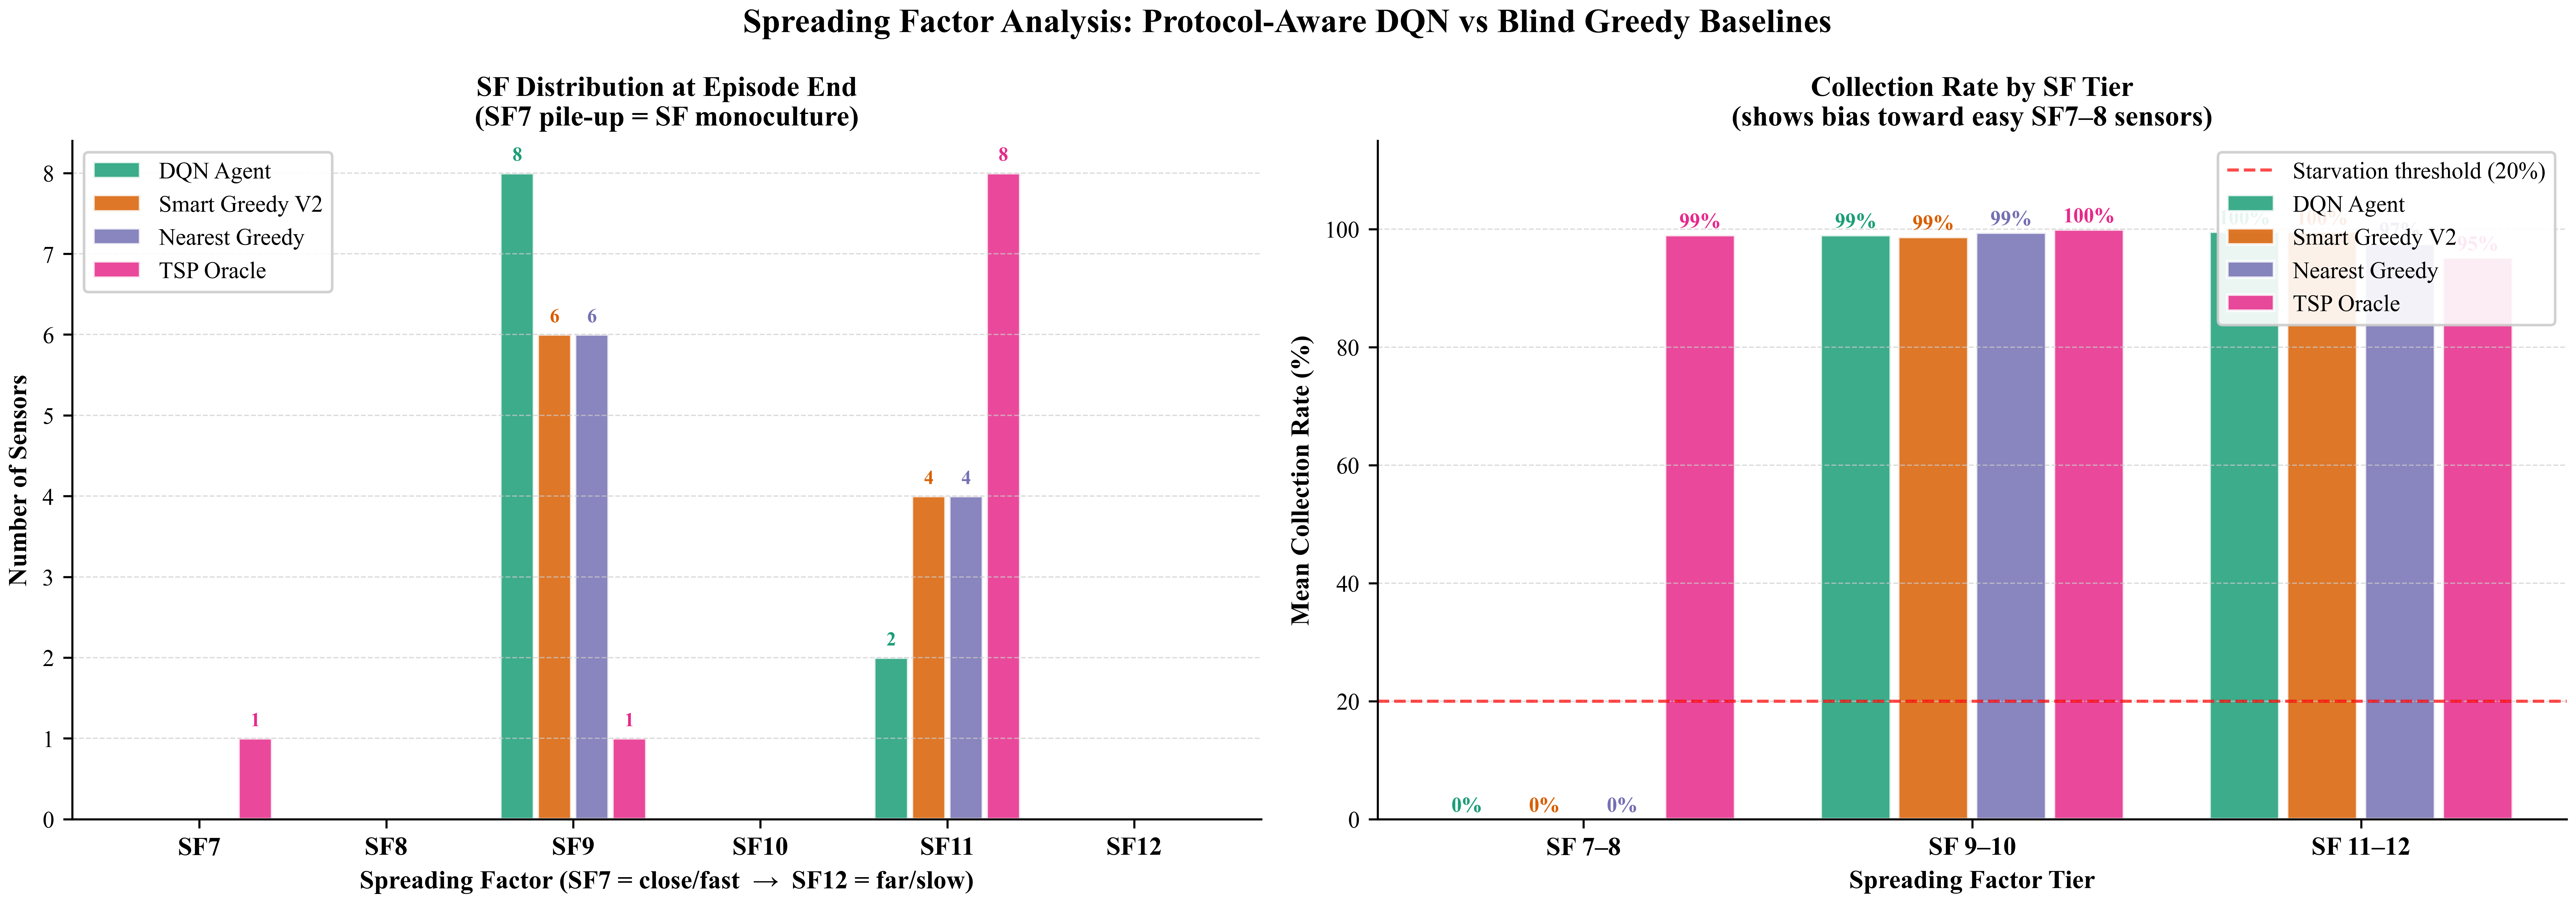
\includegraphics[width=\linewidth]{sf_distribution_vs_collection.png}
        \end{column}
        \begin{column}{0.5\textwidth}
            \centering
            
\includegraphics[width=\linewidth]{sf_monoculture_index.png}
        \end{column}
    \end{columns}
    \smallskip
    DQN systematically delays collapse onto high SFs (SF11--SF12), maintaining
    SF7--SF11 diversity longer than SF-Aware Greedy --- directly attacking the
    monoculture failure mode.
\end{frame}

\begin{frame}{Ablation Study ($500{\times}500$, $N{=}20$, $n{=}20$)}
    \small
    \begin{table}
    \centering
    \begin{tabular}{l r r r l}
        \toprule
        Condition & Rew.\ ($\times 10^5$) & $\Jfi$ & Eff. & $d$ vs.\ Full ($p$) \\
        \midrule
        Full Model         & $6.39\pm3.94$ & $0.168$ & $31.1$ & ,\ \\
        A1: No Capture     & $6.20\pm3.97$ & $0.166$ & $30.5$ & $-0.049$ ($0.881$)\\
        A2: Instant ADR    & $6.73\pm4.08$ & $0.170$ & $32.4$ & $+0.086$ ($0.769$)\\
        A3: No AoI obs.    & $6.39\pm3.94$ & $0.168$ & $31.1$ & $\phantom{-}0.000$ ($1.000$)\\
        \bottomrule
    \end{tabular}
    \end{table}

    \begin{itemize}\setlength\itemsep{0.3em}
        \item \textbf{A1 Capture Effect:} $-2.8\%$ reward; direction correct but
              $p{=}0.88$ $\Rightarrow$ physics-limited at this scale.
        \item \textbf{A2 Instant ADR:} $+6.9\%$ reward --- EMA-ADR latency is
              a real planning cost; \alert{this is an oracle upper bound},
              not a deployable target.
        \item \textbf{A3 AoI observation:} $p{=}1.0$ $\Rightarrow$ AoI shapes
              \emph{training}, not inference. Robust to sensor-urgency pipeline
              failure in deployment.
    \end{itemize}
\end{frame}

\begin{frame}{Failure Mode --- Bimodal Layouts Expose MLP Topological Blindness}
    \centering
    \begin{columns}[c]
        \begin{column}{0.5\textwidth}
            \small
            \begin{tabular}{l r l}
                \toprule
                Layout & $\Delta$ vs.\ SFGreedy & $p$ \\
                \midrule
                Grid-aligned  & \green{$+2.6\%$}  & $0.007$ \\
                Ring          & \green{$+3.0\%$}  & $0.002$ \\
                Random        & $\ \ 0\%$         & $0.88$ \\
                \alert{Bimodal (2 clusters)} & \red{$-14.0\%$}   & $<10^{-3}$\\
                \bottomrule
            \end{tabular}
        \end{column}
        \begin{column}{0.5\textwidth}
            \small
            \textbf{Observation.} DQN \emph{wins} on regular layouts, \emph{loses}
            badly on disconnected clusters.

            \smallskip
            \textbf{Diagnosis.} Fixed-capacity MLP with frame-stacked vector obs
            cannot encode \emph{sensor topology} or plan inter-cluster routing.

            \smallskip
            \textbf{Evidence.} Fine-tuning on bimodal curriculum does \emph{not}
            close the gap ($-15.1\%$ after). Architectural limit, not data.
        \end{column}
    \end{columns}
    \smallskip
    \alert{Motivates relational / attention / GNN architectures} (next slide).
\end{frame}

% ==========================================================
\section{Ongoing Work}
% ==========================================================

\begin{frame}{Ongoing: Relational \& Transformer Policies}
    \textbf{Goal.} Close the $74.4\%$ TSP-Oracle ceiling on compact layouts and
    resolve the bimodal failure by giving the policy an explicit
    sensor-set representation.

    \smallskip
    \begin{columns}[T]
        \begin{column}{0.5\textwidth}
            \textbf{1. Relational Policy (PPO + RLlib new API)}
            \begin{itemize}\setlength\itemsep{0.15em}
                \item Multi-head self-attention over sensor tokens.
                \item Permutation invariant in $N$; masked for padding up to
                      $N_{\max}{=}50$.
                \item Trains on the same 5-stage competence curriculum as DQN.
            \end{itemize}
        \end{column}
        \begin{column}{0.5\textwidth}
            \textbf{2. Transformer Policy (GTrXL + PPO)}
            \begin{itemize}\setlength\itemsep{0.15em}
                \item Gated Transformer-XL with $50$-step memory
                      $\Rightarrow$ covers $5\times$ EMA-ADR lag ($\tau{=}10$).
                \item Gated residual resolves burst-silence aliasing
                      (10\% Tx probability).
                \item 8 attention heads $\Rightarrow$ parallel urgency, ADR,
                      proximity tracking.
            \end{itemize}
        \end{column}
    \end{columns}
    \smallskip
    \textbf{Status.} Both training pipelines built and running on dual-GPU RunPod;
    curriculum-gate telemetry bug found \& fixed this session (commit \texttt{ad6a2c0}).
    Results targeted for final report.
\end{frame}

% ==========================================================
\section{Conclusions}
% ==========================================================

\begin{frame}{Key Contributions}
    \begin{enumerate}\setlength\itemsep{0.25em}
        \item \textbf{Open simulator:} first Gymnasium env modelling the full
              UAV\,$\to$\,RSSI\,$\to$\,ADR\,$\to$\,Capture\,$\to$\,delivery chain.
        \item \textbf{Curriculum DQN} generalising across all 16 conditions without
              retraining.
        \item \textbf{Novel SF-Aware Greedy + TSP Oracle} baselines;
              ceiling \alert{74.4\%} above DQN on compact grids.
        \item \textbf{Statistical parity with heuristics} on the primary condition
              ($p\!=\!0.876$, $p\!=\!0.889$).
        \item \textbf{Operational envelope:} trivial / feasible / infeasible regimes
              characterised; $1000^2$ shown \emph{physically} infeasible for a
              single UAV (tour $2.8\times$ over budget).
        \item \textbf{Emergent dwell-then-reposition:} long-horizon protocol-aware
              strategy, inaccessible to greedy look-ahead.
    \end{enumerate}
\end{frame}

\begin{frame}{Future Work}
    \begin{enumerate}\setlength\itemsep{0.4em}
        \item \textbf{Multi-UAV coordination} (QMIX / MAPPO) --- the only route
              past the single-UAV feasibility ceiling at $1000^2$.
        \item \textbf{Attention / GNN policy} --- close the 74\% TSP-Oracle gap
              and fix the bimodal failure. \alert{Training runs in progress.}
        \item \textbf{3D trajectory + continuous actions} (SAC/TD3) --- exploit
              altitude for Capture-Effect power differential.
        \item \textbf{Sim-to-Real.} Hardware-in-the-loop LoRaWAN testbed to
              quantify joint GPS + path-loss + wind-drift perturbations.
    \end{enumerate}
    \vfill
    \centering
    \Large Thank you --- questions?
\end{frame}

\end{document}
